\documentclass[apj]{emulateapj}

\newcommand{\kms}{km~s$^{-1}$}
\newcommand{\mgii}{\textrm{Mg}~\textsc{ii}}
\newcommand{\nev}{[\textrm{Ne}~\textsc{v}]}
\newcommand{\oii}{[\textrm{O}~\textsc{ii}]}
\newcommand{\oiii}{[\textrm{O}~\textsc{iii}]}
\newcommand{\msun}{M$_{\odot}$}
\newcommand{\mstar}{M$_{*}$}
\newcommand{\units}{M$_{\odot}$~yr$^{-1}$~kpc$^{-2}$}
\newcommand{\lrest}{\lambda_{\textnormal{\scriptsize{rest}}}}
\newcommand{\lobs}{\lambda_{\textnormal{\scriptsize{obs}}}}
\newcommand{\sigmasfr}{\Sigma_{\textnormal{\scriptsize{SFR}}}}
\newcommand{\sfrir}{\textnormal{SFR}_{\textnormal{\scriptsize{IR}}}}


\shorttitle{Compact Starbursts Driving High-Velocity Outflows}
\shortauthors{Diamond-Stanic et al.}

\begin{document}

\title{In the Crucible: Massive Compact Galaxies with High-Velocity
  Outflows and Eddington-Limited Star Formation}

\author{Aleksandar M. Diamond-Stanic\altaffilmark{1,2}, John
  Moustakas\altaffilmark{1}, Christy A. Tremonti\altaffilmark{3},
  Alison L. Coil\altaffilmark{1}, Ryan C. Hickox\altaffilmark{4}, Aday
  Robaina\altaffilmark{5}, Gregory H. Rudnick\altaffilmark{6}, \& Paul
  Sell\altaffilmark{3} }

\altaffiltext{1}{Center for Astrophysics and Space Sciences,
  University of California, San Diego, La Jolla, CA 92093, USA}
\altaffiltext{2}{Center for Galaxy Evolution Fellow}
\altaffiltext{3}{Department of Astronomy, University of
  Wisconsin-Madison, Madison, WI 53706, USA}
\altaffiltext{4}{Department of Physics and Astronomy, Dartmouth
  College, Hanover, NH 03755, USA} 

\altaffiltext{5}{Institut de Ci{\'e}ncies del Cosmos, University of
  Barcelona, 08028 Barcelona, Spain}

\altaffiltext{6}{Department of Physics and Astronomy, University of
  Kansas, Lawrence, KS 66045, USA}

\begin{abstract}

We present the discovery of compact, obscured star formation in
galaxies that exhibit $\gtrsim1000$~\kms\ outflows.  Using optical
morphologies from the Hubble Space Telescope and infrared photometry
from the Wide-field Infrared Survey Explorer, we estimate star
formation rate (SFR) surface densities that approach
$\sigmasfr\approx5000$~\msun~yr$^{-1}$~kpc$^{-2}$, which is comparable
to the Eddington limit from radiation pressure on dust grains.  We
argue that feedback associated with a compact starburst in the form of
radiation pressure from massive stars and ram pressure from supernovae
and stellar winds is sufficient to produce the high-velocity outflows
we observe, without the need to invoke feedback from an active
galactic nucleus.

\end{abstract}

\keywords{galaxies: evolution --- galaxies: kinematics and dynamics
  --- galaxies: ISM --- galaxies: starburst}

\section{Introduction}

The central regions of elliptical galaxies are thought to form in
compact starbursts \citep[e.g.,][]{kor09,hop09}.  Feedback associated
with such starbursts can produce outflows driven by thermal energy
from supernova explosions \citep[e.g.,][]{che85}, stellar winds
\citep[e.g.,][]{lei92}, and momentum input from both supernova ram
pressure and radiation pressure on dust grains \citep[e.g.,][]{mur05}.
It has been argued that such feedback imposes a limit on the maximum
star-formation rate surface density ($\sigmasfr$) for starbursts
\citep[e.g.,][]{leh96,meu97,mur05,tho05} and the maximum stellar
surface density for elliptical galaxies and star clusters
\citep[e.g.,][]{hop10}.

Galactic winds are ubiquitous in star-forming galaxies at all
redshifts and generally exhibit outflow velocities in the
100--500~\kms\ range
\citep[e.g.,][]{hec00,sha03,mar05,rup05,wei09,rub10,ste10}.  Thus, the
discovery of $|v|>1000$~\kms\ outflows in a sample of massive
($\textnormal{\mstar}\approx10^{11}$~\msun) post-starburst galaxies at
$z\sim0.6$ by \citet{tre07} suggested that a more energetic source,
such as feedback from an accreting supermassive black hole
\citep[e.g.,][]{sil98,dim05}, could have been responsible for
launching the winds \citep[see][for a recent review]{fab12}.

However, it also plausible that feedback from a compact starburst
could expel gas with such large velocities.  Indeed, there is evidence
for a positive correlation between outflow velocity and starburst
luminosity \citep[e.g.,][]{mar05,rup05,tre07}, albeit with significant
scatter.  Furthermore, \citet{hec11} recently found outflows with
maximum velocities reaching $-1500$~\kms\ in a sample of local
starbursts with compact nuclei, and argued that such velocities could
be explained by feedback from massive stars.


In this Letter, we present results for a sample of massive galaxies at
$z\sim0.6$ that exhibit $\gtrsim1000$~\kms\ outflows, expanding on the
sample from \citet{tre07}.  We seek to test whether the energetic
outflows in these galaxies could have been driven by feedback from
starbursts with very large star-formation rate (SFR) surface densities
($\sigmasfr$).  Our analysis combines galaxy sizes obtained with the
Hubble Space Telescope (HST) with star-formation rates and stellar
masses estimated using photometry from the Wide-field Infrared Survey
Explorer (WISE), the Spitzer Space Telescope, the Sloan Digital Sky
Survey (SDSS), and the Galaxy Evolution Explorer (GALEX).


\begin{figure}[!t]
\includegraphics[angle=0,scale=0.41]{3seds.ps}
\caption{Left: Observed UV--IR SEDs ($\lrest=0.1$--15~$\mu$m) for
  three galaxies with large SFR surface densities
  ($\sigmasfr>3000$~\units).  We show stellar population fits to the
  $\lrest=0.1$--3~$\mu$m emission (black solid line) and two templates
  for dust emission \citep[M82 starburst, Arp 220 starburst;][]{pol07}
  scaled to match the $\lobs=4.6~\mu$m band.  The starburst templates
  provide reasonable fits to the $\lobs=12$ and 22~$\mu$m WISE
  photometry, while a quasar template does not.  Right: HST/WFC3 F814W
  images (probing $\lrest\approx5000$~\AA) showing that these galaxies
  are dominated by a compact nucleus.}
\label{fig:seds}
\end{figure}


\section{Analysis}

\subsection{Morphologies and Sizes}

Our sample derives from 29 galaxies targeted for HST/WFC3 imaging in
programs 12019 and 12272 (PI: C. Tremonti).  Using the F814W filter on
the UVIS channel, which has $0.04\arcsec$ pixels and
$\textnormal{FWHM}=0.074\arcsec$, we obtained $4\times10$~min
exposures in a single orbit for each galaxy.  The dithered images were
processed with
MultiDrizzle\footnote{http://stsdas.stsci.edu/multidrizzle/} to
produce science mosaics with $0.02\arcsec$ pixels.  For each galaxy,
we use GALFIT \citep{pen02} to model the two-dimensional surface
brightness profile with a single Sersic component, using stars in the
images to construct the model point-spread function (PSF).  The Sersic
index (n) and effective radius ($r_e$) are free parameters in the
model.  In cases where the best-fit model returns $n>4$, we also fit
an $n=4$ de Vaucouleurs model, yielding a larger $r_e$ value (due to
the covariance between $n$ and $r_e$), and we use these these larger
effective radii in our analysis.

For this paper, we are most interested in the galaxies with the
largest $\sigmasfr$ values, which also have the smallest effective
radii.  We show the HST images for three high-$\sigmasfr$ galaxies in
Figure~\ref{fig:seds}.  In all three cases, the single-component model
GALFIT accounts for $>85\%$ of the total flux.  The residuals show
diffuse emission that is consistent with these systems being
late-stage galaxy mergers after final coalescence, although we defer a
detailed comparison of the observed morphologies with expectations
from merger simulations to future work.

For the most compact galaxy (J0905+5759, $r_e=0.013\arcsec$ or
100~pc), we also show the observed one-dimensional surface brightness
profile in the bottom-right panel of Figure~\ref{fig:profile}.  We
compare to the profiles of six stars in the same image, the best-fit
de Vaucouleurs model, and a de Vaucouleurs model with a larger
effective radius ($r_e=0.04\arcsec$, the native WFC3/UVIS pixel size,
which corresponds to a physical scale of 290~pc).  This comparison
illustrates that this galaxy, while only marginally resolved with an
effective radius that is $\sim20\%$ of the image FWHM, is clearly more
extended than a point source.

For such a compact source, there is significant uncertainty in our
$r_e$ measurement given uncertainties in the model PSF.  To quantify
this uncertainty, we used TinyTim to generate a model PSF that is
artificially narrower than the stars in the image (convolving the
output of tiny2 with a $\textnormal{FWHM}=0.04\arcsec$ Gaussian,
whereas the image FWHM is $0.074\arcsec$) and found that this
increased the effective radius in the GALFIT model by a factor of two.
We also fit a two-component PSF+Sersic model, but found that the
Sersic component dominates the fit, yielding a similar effective
radius.  Furthermore, the spectrum of the galaxy shows no evidence for
an AGN contribution to the $I$-band continuum (see
Figure~\ref{fig:spectra}), so there is no clear motivation for
including an unresolved, point-source component in the model.  We
conclude that this galaxy is quite compact and that our $r_e$ estimate
of 100~pc, while uncertain, is likely accurate within a factor of two.

\begin{figure}[!t]
\includegraphics[angle=0,scale=0.41]{profile.ps}
\label{fig:profile}
\caption{One-dimensional surface brightness profile for J0905+5759,
  which has the smallest effective radius in the sample.  The observed
  profile is shown as the solid black line, and the profiles of six
  stars in the same image are shown in blue.  The best-fit de
  Vaucouleurs profile with $r_e=100$~pc is shown as a dashed red line,
  and for comparison a broader profile with $r_e=0.04\arcsec=290$~pc
  is shown as the dotted green line.  This galaxy is quite compact,
  but is more extended than a point source.}
\end{figure}

\subsection{Star Formation Rates and Stellar Masses}

% We gathered photometry from the All-Sky Release of the Wide-field
% Infrared Survey Explorer \citep[WISE,][]{wri10}, the Seventh Data
% Release of the Sloan Digital Sky Survey \citep[SDSS,][]{aba09}, and
% General Release 6 from the Galaxy Evolution Explorer
% \citep[GALEX,][]{mar05galex}.  
We gathered photometry from the WISE All-Sky Release, the SDSS Seventh
Data Release, and GALEX General Release 6.  We also obtained
$5\times30$~sec dithered exposures at 3.6~$\mu$m and 4.5~$\mu$m for
all sources with the Infrared Array Camera on the Spitzer Space
Telescope as part of General Observer program 60145 (PI: C. Tremonti).
We used the post--basic calibrated data to perform aperture photometry
on all sources, and we also used the
APEX\footnote{http://irsa.ipac.caltech.edu/data/SPITZER/docs/dataanalysistools/tools/mopex/}
point-source extraction software for photometry of sources in crowded
fields.  We show spectral energy distributions (SEDs) for the three
high-$\sigmasfr$ galaxies in Figure~\ref{fig:seds}.

% All the photometry was corrected for Galactic extinction
% based on the \citet{sch98} dust maps.

We estimate IR-based star-formation rates for the 25/29 galaxies with
WISE 12 or 22~$\mu$m detections by fitting \citet{cha01} templates to
their 12 and 22~$\mu$m fluxes.  For the 14/29 galaxies with 22~$\mu$m
detections, this yields SFRs that agree with those obtained from the
\citet{ruj12} method based on 24~$\mu$m luminosity with a scatter of
0.05~dex.  We note that several authors have shown that the shape of
the IR SED for star-forming galaxies depends on the surface density of
star formation \citep[e.g.,][]{ruj11,elb11}, with more compact
starbursts having larger total-IR (8--1000~$\mu$m) to mid-IR
(8--24~$\mu$m) ratios.  The extreme $\sigmasfr$ values of our sample
imply large total-IR to mid-IR ratios, characteristic of the most
luminous galaxies in the local universe
\citep[e.g.,][]{rie09}.  If we used the most luminous
local templates for the 8/29 sources with SFRs in the ULIRG regime
($\sfrir>200$~\msun~yr$^{-1}$), we would obtain SFRs that are larger
by 0.5~dex than the values we adopt for this paper.

We also estimate star-formation rates and stellar masses based on
stellar population fits to the $\lrest=0.1$--3~$\mu$m SEDs using the
method of \citet{mou11}.  For galaxies with
$\sfrir>50$~\msun~yr$^{-1}$, there is agreement between these UV-based
SFR estimates and $\sfrir$ with a scatter of 0.32~dex.  For an SMC
dust law, we find a median attenuation of $A_V=0.4$~mag.

\begin{figure}[!t]
\includegraphics[angle=0,scale=0.41]{spectra.ps}
\caption{Spectra covering $\lrest=2500$--5200~\AA\ for the three
  galaxies shown in Figure~\ref{fig:seds}.  These spectra are
  dominated by light from the young stellar population and exhibit
  \oii~$\lambda3727$, H$\beta$~$\lambda4861$, and \oiii~$\lambda5007$
  emission lines.  The panels on the right highlight the
  \mgii~$\lambda\lambda2796,2803$ spectral region in both wavelength
  and velocity space to illustrate the outflow kinematics.  The
  spectrum in the bottom panel has sufficient spectral resolution
  ($\textnormal{FWHM}\approx8$~\kms) to resolve the intrinsic shape of
  the absorption-line profile, revealing that the gas near the
  centroid velocity ($v=-2470$~\kms) covers the entire galaxy.}
\label{fig:spectra}
\end{figure}

\begin{figure*}[!t]
\begin{center}
\includegraphics[angle=0,scale=.8]{sigmasfr.ps} 
\caption{SFR surface densities and stellar masses for the HST--WISE
  sample described in this paper (black circles, with symbol size
  proportional to outflow velocity), along with samples of gas-rich
  mergers (orange squares) and star-forming galaxies (shown with 68\%,
  95\%, and 99.7\% contours).  We mark the empirical threshold for
  launching winds \citep[dotted line,
    $\sigmasfr\approx0.1$~\units;][]{hec02}, the 90th-percentile
  starburst intensity limit from \citet{meu97} (dashed line,
  $\sigmasfr\approx45$~\units), and the Eddington limit from radiation
  pressure on dust grains \citep[solid line,
    $\sigmasfr\approx2000$~\units;][]{mur05,tho05,hop10}.  Our
  HST--WISE sample overlaps with the region characterized by gas-rich
  mergers, and extends to very large SFR surface densities near the
  Eddington limit, suggesting growth that is limited by momentum
  injection from massive stars.}
\label{fig:sigmasfr}
\end{center}
\end{figure*}

\subsection{Outflow Kinematics and Covering Factors}

We present $\lrest=2500$--5200~\AA\ spectroscopy for three
high-$\sigmasfr$ sources in Figure~\ref{fig:spectra} based on data
from MMT/Blue Channel and SDSS (J1506+5402), Magellan/MAGE
(J1341-0321), and Keck/LRIS and Keck/HIRES (J0905+5759).  The spectra
are dominated by light from the young ($t<50$~Myr) stellar population.
We highlight the \mgii~$\lambda\lambda2796,2803$ absorption lines,
which are used used to measure outflow velocities.  At low spectral
resolution (e.g., the top right panel of Figure~\ref{fig:spectra}) it
is not possible to determine the intrinsic shape of the absorption
line profile and therefore the covering factor of the outflowing gas.
However, the Keck/HIRES spectrum of J0905+5759
($\textnormal{FWHM}\approx8$~\kms) reveals that the gas covers the
entire continuum source near the velocity centroid ($v=-2470$~\kms)
indicating a galaxy-wide outflow.


\section{Discussion}

The compact sizes ($r_e\approx100$~pc) and large star formation rates
($\textnormal{SFR}\approx300$~\msun) for the galaxies described above
implies extremely large star-formation rate surface densities
($\sigmasfr\approx5000$~\units).  To place these galaxies in context,
we plot their $\sigmasfr$ values as a function of stellar mass in
Figure~\ref{fig:sigmasfr}.  We include comparison samples of
$\sim10^5$ star-forming galaxies at $0.5<z<1.5$ from \citet{wuy11} and
a few dozen gas-rich mergers at $z<0.3$ including 32 ULIRGs from
\citet{vei06}, five Lyman break analogs with dominant central objects
from \citet{ove09}, and the local compact starburst Arp 220
\citep{sco97, ken98, rod08}.  We also mark the empirical threshold for
launching winds \citep[$\sigmasfr\approx0.1$~\units,][]{hec02}, the
90th percentile limit for the surface brightness of starbursts
measured using UV, H$\alpha$, far-IR, and radio continuum emission
\citep[$\sigmasfr\approx45$~\units][]{meu97}, and the theoretical
limit for a starburst limited by feedback from radiation pressure
\citep[$\sigmasfr\approx2000$~\units,][]{mur05,tho05,hop10}.  The most
luminous, compact starbursts in our sample exhibit SFR surface
densities that reach the Eddington limit, suggesting that their growth
is being regulated by momentum input from massive stars.


\subsection{Constraints on Ongoing AGN Activity}

While the SEDs (Figure~\ref{fig:seds}) and optical spectra
(Figure~\ref{fig:spectra}) for our sample indicate that their
bolometric output is dominated by star formation, it is worthwhile to
consider the level of ongoing AGN activity and its effect on our
measurements.  Among the high-$\sigmasfr$ galaxies, the strongest case
for detectable AGN emission can be made for J1506+5402, which has the
most luminous \oiii~$\lambda5007$ line among the 29 galaxies observed
by HST.  This source also has a weak \nev~$\lambda3426$ emission line,
which is associated with AGN activity \citep[e.g.,][]{gil10}.  It was
observed with the Chandra X-ray Observatory (proposal ID 11700896, PI:
C. Tremonti) and had four detected counts, corresponding to a
0.5--8.0~keV X-ray luminosity of $10^{42.7}$~erg~s$^{-1}$ (see P. Sell
et al., in preparation for more details on the 12/29 galaxies with
Chandra observations).  Using the relationship between 2--10~keV X-ray
and 12.3~$\mu$m mid-IR luminosity for AGNs from \citet{gan09}, one
would expect a source with
$L_{\textnormal{\scriptsize{X}}}\approx5\times10^{42}$~erg~s$^{-1}$ to
have
$L_{\textnormal{\scriptsize{MIR}}}\approx7\times10^{42}$~erg~s$^{-1}$,
which is 400$\times$ smaller than observed luminosity for J1506+5402
($L_{\textnormal{\scriptsize{MIR}}}\approx3\times10^{45}$~erg~s$^{-1}$).
Based on its \oiii\ luminosity ($10^{42.1}$~erg~s$^{-1}$, a
significant fraction of which could be attributed to star formation)
and the calibration for type 1 AGNs from \citet{hec05}, one would
expect an intrinsic 2--10~keV luminosity of
$L_{\textnormal{\scriptsize{X}}}\approx5\times10^{43}$~erg~s$^{-1}$,
suggesting absorption by a factor of $\sim10$ in the X-rays.  However,
even if the X-ray attenuation were a factor of 100, which is the
typical value for local Compton-thick AGNs \citep{dia09}, the expected
mid-IR AGN contribution would only be relevant at the $\lesssim$30\%
level.  We conclude that the bolometric output of the galaxies in our
sample is dominated by star and we that our results regarding large
$\sigmasfr$ values are not affected by AGN contamination.

% Thus, similar to local ULIRGs \citep[e.g.,][]{far07}, the
% bolometric output of the galaxies in our sample is dominated by star
% formation, and we conclude that our results regarding large
% $\sigmasfr$ values are not affected by AGN contamination.


\subsection{The Outflow Launching Mechanism}\label{sec:launch}

It is worth considering whether the high-velocity outflows we observe
were produced by the compact starburst.  \citet{mur11} argued that
massive star clusters with large gas surface densities are the ideal
launching point for galactic-scale outflows driven by radiation
pressure, and that the outflow velocity should scale with escape
velocity of the most massive star clusters in a galaxy.  The
$\gtrsim1000$~\kms\ outflow velocities we observe correspond
approximately to the escape velocities for a compact stellar
population with the sizes and masses that we've measured.
\begin{eqnarray}\nonumber
v_{esc}&=&\sqrt{2GM_{*}/r} \\
&=& 2100
\left({M_{*}\over10^{11} M_{\odot}}\right)^{1/2} 
\left({r\over200~\textnormal{pc}}\right)^{-1/2}
\textnormal{km~s}^{-1} 
\label{eq:vesc}
\end{eqnarray}
This argument, combined with the fact that we observe galaxies with
significant dust-obscured star formation and $\sigmasfr$ values near
the Eddington limit, indicates that momentum input from massive stars
in the form of radiation pressure is a viable mechanism for launching
these outflows.

In addition to radiation pressure, we also expect significant momentum
flux from stellar winds and supernovae.  For example, a starburst with
$\textnormal{SFR}\approx200$~\msun~yr$^{-1}$ would be associated with
radiation pressure $L_{bol}/c\approx2\times10^{35}$~dyne and ram
pressure $\dot{p}\approx5$--$10\times10^{35}$~dyne from stellar winds
and supernovae \citep[e.g.,][]{lei92,lei99,vei05}.  Furthermore,
\citet{hec11} noted that such a large momentum injection
($\dot{p}\approx10^{35}$~dyne) from a small initial radius
$r_{0}\approx100$~pc could accelerate a cloud with column density
$N_{H}\approx10^{21}$~cm$^{-2}$ to a terminal velocity
$v_{\infty}\approx1800$~\kms.  Thus, the energetics of compact
starbursts are sufficient to produce the high-velocity outflows we
observe, and it is plausible that both radiation pressure on dust
grains and supernova ram pressure contribute to driving the winds.


\subsection{Placing These Galaxies in Context}

It is clear from Figure~\ref{fig:sigmasfr} that the high-$\sigmasfr$
galaxies in our sample constitute a rare population, suggesting that
they represent an unusual or short-lived phase.  Mergers of gas-rich
galaxies are a viable mechanism for producing compact starbursts
\citep[e.g.,][]{mih96}, and such gas-rich major mergers are rare at
$z\sim0.6$ due to the decline in both the merger rate
\citep[e.g.,][]{lot11} and the gas fraction \citep[e.g.,][]{tac10} of
galaxies since $z\sim2$.  Furthermore, the high-$\sigmasfr$ galaxies
are caught in a particular time interval where there is both vigorous
star formation and strong feedback.  The length of this phase may be
set by the gas consumption timescale or the timescale for feedback to
suppress subsequent star formation.  Based on the Kennicutt--Schmidt
(K-S) relation \citep{ken98}, a compact starburst with
$r_e\approx100$~pc, $\textnormal{SFR}\approx300$~\msun, and
$\sigmasfr\approx5000$~\units\ would have a gas surface density of
$\Sigma_{gas}\sim2\times10^{11}$~\msun~kpc$^{-2}$ corresponding to
$M_{gas}\sim5\times10^{9}$~\msun\ inside 100~pc, which would be
consumed on a timescale $\sim30$~Myr.  This scenario could be tested
with CO observations of molecular gas masses and kinematics for these
extreme galaxies.


Considering our full sample of galaxies in Figure~\ref{fig:sigmasfr},
a vertical $\sigmasfr$ sequence is apparent.  This could be explained
as an evolutionary sequence where the high-$\sigmasfr$ galaxies
represent the peak of the starburst where the high-velocity outflows
are launched, while the lower $\sigmasfr$ galaxies represent a
subseqent, post-starburst phase.  It is interesting to note that all
12/29 galaxies above the $\sigmasfr\approx45$~\units\ limit from
\citet{meu97} exhibit outflows (with median centroid velocity
$v=-1500$~\kms), while all 7/29 galaxies without detected outflows
have $\sigmasfr<30$~\units.  If a compact starburst is a requirement
for the production of high-velocity outflows, it may be that the
sources without outflows have not gone through such a phase (see
A. Robaina, et al., in preparation for a discussion of the
relationship between galaxy morphology, outflow velocity, and stellar
population age in this sample).

Finally, it is worthwhile to consider the implications of our results
for models of massive galaxy formation.  Simulaitons of major galaxy
mergers with large gas fractions ($f_{gas}\sim50$\%) can produce
$\textnormal{\mstar}\sim10^{11}$~\msun\ remnants with effective radii
$r_{e}\sim1$~kpc \citep[e.g.,][]{wuy10}, but our sample includes
galaxies of similar mass that are smaller by almost an order of
magnitude.  If these systems do evolve into quiescent elliptical
galaxies, it would be quite challenging for them to grow in size from
$r_e\sim0.1$~kpc to $r_e\sim5$~kpc to reach the local size--mass
relation \citep{she03} in the $t\sim6$~Gyr since $z=0.6$.  For
comparison the compact, quiescent galaxies observed at $z\sim2$
\citep[e.g.,][]{tru07,van08} have $t\sim10$~Gyr to grow by a factor of
$\sim5$.  In this context, it is worth noting that the half-light
radius (ignoring dust attenuation) at rest-frame $V$ band (where our
HST observations probe) can be a factor of 5--10 smaller than the
half-mass radius for a gas-rich merger at final coalescence near the
peak of starburst activity \citep{wuy10}.  It would be worthwhile to
test for such size discrepancies and to pronbe the radial dependence
of the mass-to-light ratio for these galaxies by measuring sizes at
rest-frame near-IR wavelengths.

 

\section{Conclusions}

We have measured large SFR surface densities for galaxies that exhibit
$\gtrsim1000$~\kms\ outflows.  The largest $\sigmasfr$ values are
comparable to the Eddington limit from radiation pressure on dust
grains, and such compact starburst are expected to have substantial
momentum input from both massive stars and supernovae.  There is some
evidence for AGN activity in a fraction of these systems, but the AGN
is generally not relevant in a bolometric sense.  High-velocity
outflows have been previously interpreted as a signpost of AGN
feedback, but we conclude that stellar feedback from a compact
starburst is equally capable of producing such a signature.


\acknowledgments

We acknowledge useful discussions with and assistance from several
people.  AMD acknowledges support from the Southern California Center
for Galaxy Evolution, a multi-campus research program funded by the
University of California Office of Research.


\begin{thebibliography}{}
%\bibitem[Abazajian et al.(2009)]{aba09} Abazajian, K.~N.,
%  Adelman-McCarthy, J.~K., Ag{\"u}eros, M.~A., et al.\ 2009, \apjs,
%  182, 543
%\bibitem[Abel \& Satyapal(2008)]{abe08} Abel, N.~P., \& Satyapal,
%  S.\ 2008, \apj, 678, 686
\bibitem[Chary \& Elbaz(2001)]{cha01} Chary, R., \& Elbaz, D.\ 2001,
  \apj, 556, 562
\bibitem[Chevalier \& Clegg(1985)]{che85} Chevalier, R.~A., \& Clegg,
  A.~W.\ 1985, \nat, 317, 44
%\bibitem[Dale \& Helou(2002)]{dal02} Dale, D.~A., \& Helou, G.\ 2002,
%  \apj, 576, 159
%\bibitem[de Vaucouleurs(1948)]{dev48} de Vaucouleurs, G.\ 1948,
%  Annales d'Astrophysique, 11, 247
%\bibitem[Debuhr et al.(2012)]{deb12} Debuhr, J., Quataert, E., \& Ma,
%  C.-P.\ 2012, \mnras, 420, 2221
\bibitem[Diamond-Stanic et al.(2009)]{dia09} Diamond-Stanic, A.~M.,
  Rieke, G.~H., \& Rigby, J.~R.\ 2009, \apj, 698, 623
\bibitem[Di Matteo et al.(2005)]{dim05} Di Matteo, T., Springel, V.,
  \& Hernquist, L.\ 2005, \nat, 433, 604
\bibitem[Elbaz et al.(2011)]{elb11} Elbaz, D., Dickinson, M., Hwang,
  H.~S., et al.\ 2011, \aap, 533, A119
\bibitem[Fabian(2012)]{fab12} Fabian, A.~C.\ 2012,
  arXiv:1204.4114
%\bibitem[Farrah et al.(2007)]{far07} Farrah, D., Bernard-Salas, J.,
%  Spoon, H.~W.~W., et al.\ 2007, \apj, 667, 149
%\bibitem[Fazio et al.(2004)]{faz04} Fazio, G.~G., Hora, J.~L., Allen,
%x  L.~E., et al.\ 2004, \apjs, 154, 10
\bibitem[Gandhi et al.(2009)]{gan09} Gandhi, P., Horst, H., Smette,
  A., et al.\ 2009, \aap, 502, 457
\bibitem[Gilli et al.(2010)]{gil10} Gilli, R., Vignali, C., Mignoli,
  M., et al.\ 2010, \aap, 519, A92
%\bibitem[Heckman et al.(1993)]{hec93} Heckman, T.~M., Lehnert, M.~D.,
%  \& Armus, L.\ 1993, The Environment and Evolution of Galaxies, 188,
%  455
\bibitem[Heckman et al.(2000)]{hec00} Heckman, T.~M., Lehnert, M.~D.,
  Strickland, D.~K., \& Armus, L.\ 2000, \apjs, 129, 493
\bibitem[Heckman(2002)]{hec02} Heckman, T.~M.\ 2002, Extragalactic Gas
  at Low Redshift, 254, 292
\bibitem[Heckman et al.(2005)]{hec05} Heckman, T.~M., Ptak, A.,
  Hornschemeier, A., \& Kauffmann, G.\ 2005, \apj, 634, 161
\bibitem[Heckman et al.(2011)]{hec11} Heckman, T.~M., et al.\ 2011,
  \apj, 730, 5
\bibitem[Hopkins et al.(2009)]{hop09} Hopkins, P.~F., Cox, T.~J.,
  Dutta, S.~N., et al.\ 2009, \apjs, 181, 135
\bibitem[Hopkins et al.(2010)]{hop10} Hopkins, P.~F., Murray, N.,
  Quataert, E., \& Thompson, T.~A.\ 2010, \mnras, 401, L19
\bibitem[Kennicutt(1998)]{ken98} Kennicutt, R.~C., Jr.\ 1998, \apj,
  498, 541
\bibitem[Kormendy et al.(2009)]{kor09} Kormendy, J., Fisher, D.~B.,
  Cornell, M.~E., \& Bender, R.\ 2009, \apjs, 182, 216
\bibitem[Lehnert \& Heckman(1996)]{leh96} Lehnert, M.~D., \& Heckman,
  T.~M.\ 1996, \apj, 472, 546
\bibitem[Leitherer et al.(1992)]{lei92} Leitherer, C., Robert, C., \&
  Drissen, L.\ 1992, \apj, 401, 596
\bibitem[Leitherer et al.(1999)]{lei99} Leitherer, C., Schaerer, D.,
  Goldader, J.~D., et al.\ 1999, \apjs, 123, 3
\bibitem[Lotz et al.(2011)]{lot11} Lotz, J.~M., Jonsson, P., Cox,
  T.~J., et al.\ 2011, \apj, 742, 103
\bibitem[Martin(2005)]{mar05} Martin, C.~L.\ 2005, \apj, 621, 227
%\bibitem[Martin et al.(2005)]{mar05galex} Martin, D.~C., Fanson, J.,
%  Schiminovich, D., et al.\ 2005, \apjl, 619, L1
\bibitem[Meurer et al.(1997)]{meu97} Meurer, G.~R., Heckman, T.~M.,
  Lehnert, M.~D., Leitherer, C., \& Lowenthal, J.\ 1997, \aj, 114, 54
\bibitem[Mihos \& Hernquist(1996)]{mih96} Mihos, J.~C., \& Hernquist,
  L.\ 1996, \apj, 464, 641
\bibitem[Moustakas et al.(2011)]{mou11} Moustakas, J., Zaritsky, D.,
  Brown, M., et al.\ 2011, arXiv:1112.3300
\bibitem[Murray et al.(2005)]{mur05} Murray, N., Quataert, E., \&
  Thompson, T.~A.\ 2005, \apj, 618, 569
\bibitem[Murray et al.(2011)]{mur11} Murray, N., M{\'e}nard, B., \&
  Thompson, T.~A.\ 2011, \apj, 735, 66
\bibitem[Overzier et al.(2009)]{ove09} Overzier, R.~A., Heckman,
  T.~M., Tremonti, C., et al.\ 2009, \apj, 706, 203
\bibitem[Peng et al.(2002)]{pen02} Peng, C.~Y., Ho, L.~C., Impey,
  C.~D., \& Rix, H.-W.\ 2002, \aj, 124, 266
%\bibitem[Peng et al.(2010)]{pen10} Peng, C.~Y., Ho, L.~C., Impey,
%  C.~D., \& Rix, H.-W.\ 2010, \aj, 139, 2097
\bibitem[Polletta et al.(2007)]{pol07} Polletta, M., Tajer, M.,
  Maraschi, L., et al.\ 2007, \apj, 663, 81
\bibitem[Rodr{\'{\i}}guez Zaur{\'{\i}}n et al.(2008)]{rod08}
  Rodr{\'{\i}}guez Zaur{\'{\i}}n, J., Tadhunter, C.~N., \&
  Gonz{\'a}lez Delgado, R.~M.\ 2008, \mnras, 384, 875
\bibitem[Rieke et al.(2009)]{rie09} Rieke, G.~H., Alonso-Herrero, A.,
  Weiner, B.~J., et al.\ 2009, \apj, 692, 556
\bibitem[Rubin et al.(2010)]{rub10} Rubin, K.~H.~R., Weiner, B.~J.,
  Koo, D.~C., Martin, C.~L., Prochaska, J.~X., Coil, A.~L., \& Newman,
  J.~A.\ 2010, \apj, 719, 1503
\bibitem[Rujopakarn et al.(2011)]{ruj11} Rujopakarn, W.,
  Rieke, G.~H., Eisenstein, D.~J., \& Juneau, S.\ 2011, \apj, 726, 93
\bibitem[Rujopakarn et al.(2012)]{ruj12} Rujopakarn, W., Rieke, G.~H.,
  Weiner, B.~J., et al.\ 2011, arXiv:1107.2921
\bibitem[Rupke et al.(2005)]{rup05} Rupke, D.~S., Veilleux, S., \&
  Sanders, D.~B.\ 2005, \apjs, 160, 115 
%\bibitem[Schlegel et al.(1998)]{sch98} Schlegel, D.~J., Finkbeiner,
%  D.~P., \& Davis, M.\ 1998, \apj, 500, 525
\bibitem[Scoville et al.(1997)]{sco97} Scoville, N.~Z., Yun, M.~S., \&
  Bryant, P.~M.\ 1997, \apj, 484, 702
\bibitem[Shapley et al.(2003)]{sha03} Shapley, A.~E., Steidel, C.~C.,
  Pettini, M., \& Adelberger, K.~L.\ 2003, \apj, 588, 65
\bibitem[Shen et al.(2003)]{she03} Shen, S., Mo, H.~J., White,
  S.~D.~M., et al.\ 2003, \mnras, 343, 978
\bibitem[Silk \& Rees(1998)]{sil98} Silk, J., \& Rees, M.~J.\ 1998,
  \aap, 331, L1
\bibitem[Steidel et al.(2010)]{ste10} Steidel, C.~C., Erb, D.~K.,
  Shapley, A.~E., Pettini, M., Reddy, N., Bogosavljevi{\'c}, M.,
  Rudie, G.~C., \& Rakic, O.\ 2010, \apj, 717, 289
\bibitem[Tacconi et al.(2010)]{tac10} Tacconi, L.~J., Genzel, R.,
  Neri, R., et al.\ 2010, \nat, 463, 781
\bibitem[Thompson et al.(2005)]{tho05} Thompson, T.~A., Quataert, E.,
  \& Murray, N.\ 2005, \apj, 630, 167
\bibitem[Tremonti et al.(2007)]{tre07} Tremonti, C.~A., Moustakas, J.,
  \& Diamond-Stanic, A.~M.\ 2007, \apjl, 663, L77
\bibitem[Trujillo et al.(2007)]{tru07} Trujillo, I., Conselice, C.~J.,
  Bundy, K., et al.\ 2007, \mnras, 382, 109
\bibitem[van Dokkum et al.(2008)]{van08} van Dokkum, P.~G., et
  al.\ 2008, \apjl, 677, L5
\bibitem[Veilleux et al.(2005)]{vei05} Veilleux, S., Cecil, G., \&
  Bland-Hawthorn, J.\ 2005, \araa, 43, 769
\bibitem[Veilleux et al.(2006)]{vei06} Veilleux, S., Kim, D.-C., Peng,
  C.~Y., et al.\ 2006, \apj, 643, 707
\bibitem[Weiner et al.(2009)]{wei09} Weiner, B.~J., et al.\ 2009,
  \apj, 692, 187
%\bibitem[Werner et al.(2004)]{wer04} Werner, M.~W., Roellig, T.~L.,
%  Low, F.~J., et al.\ 2004, \apjs, 154, 1
%\bibitem[Wright et al.(2010)]{wri10} Wright, E.~L., Eisenhardt,
%  P.~R.~M., Mainzer, A.~K., et al.\ 2010, \aj, 140, 1868
\bibitem[Wuyts et al.(2010)]{wuy10} Wuyts, S., Cox, T.~J., Hayward,
  C.~C., et al.\ 2010, \apj, 722, 1666
\bibitem[Wuyts et al.(2011)]{wuy11} Wuyts, S., F{\"o}rster Schreiber,
  N.~M., van der Wel, A., et al.\ 2011, \apj, 742, 96
\end{thebibliography}



\end{document}

